\documentclass{article}

\usepackage{geometry}
\usepackage{float}
\usepackage{caption}
\geometry{a4paper}
\usepackage{amsmath}
\usepackage{graphicx}
\usepackage[obeyspaces]{url}
\usepackage{listings}
\usepackage[space]{grffile}
\usepackage[toc,page]{appendix}
\usepackage{comment}
\usepackage{float}

\title{Final Report\\
Prediction of Crime Patterns in Chicago using Network Analysis\vfill{}}

\author{Submitted By:\\Ravisutha Sakrepatna Srinivasamurthy\\
						Saroj Kumar Dash}

\begin{document}
	\begin{titlepage}
		\maketitle
		\pagenumbering{gobble}
		\end{titlepage}
	
\newpage

\tableofcontents

\newpage	

\pagenumbering{arabic}

\section{Introduction}
In this project we analyzed the Chicago Crime Data \cite{data} and used the dynamic data of Chicago crimes to build a network and predict the next trend in crimes. Following sections explains our objective, datasets, our approach and our findings.

\section{Objective}
Our objective is to to predict crime pattern in Chicago city by using data from previous years with the help of network analysis techniques. In order to validate our results, we are using 2015's data as the validation dataset.

\section{Dataset}
The dataset spans from a time period of 2001 to present. Since the data is produced by a government agency, data can be relied upon for its correctness. The 15 years old dataset of crimes describes about all the crime events that have happened in Chicago area. There are many analysis done on this datasets before but most of the analysis are in the traditional ways of qualitative or quantitative statistical analysis of the dataset. Our analysis is different as we try to view the dataset in form of a network and use network science concepts to extract features from it. 
\subsection{Dataset Description}
Below is a list all the data sources that we used. The most challenging part of the project was to make connections between the various parts of the crime dataset and also among all other datasets obtained from other departments. Dataset Sources:
\begin{itemize}
	\item Crime dataset\cite{crime}: Chicago crime data from 2001 to present.
	\item Chicago Library Data\cite{library_loc}  Library locations and details with map coordinates.
	\item Library visitors by location\cite{library_data}: This data gives information about the number of visitors for all libraries in Chicago city.
	\item Police Station Data\cite{police_stations}: Gives us information about the location of a police station.
	\item Police Districts Boundaries\cite{policeloc}: This data tells about the areas for which a police station is responsible for. Used to connect communities, crimes and police stations closest to it.
	\item 311 Service requests\cite{sanity}: A set of datasets for all sanitation queries.
	\item Chicago public School progress Information\cite{school} :  Data was available from 2011 to 2017.
\end{itemize} 
The main challenge in the project was to accumulate the data from each time line because there were lot of data which were not available for some years. Only the crime data could be traced back from 2001. But only a few were available from 2001. But all datasets were available from 2001. Hence dataset from 2011 to 2015 was used as training  dataset. 2015 was used for validating the data model.
\subsection{Data Cleaning}
We cleaned the data and filtered the data according to months for each year (2011-2015). We add a new column called community based on the location information from the dataset if the community info was not directly available.

\section{Approach}
Chicago city can be divided into 77 communities. Each node is considered as a node. According to Chicago Police Dept., crimes can be categorized into 401 types. We considered each crime type as a node. Crime dataset had the crime location information. Hence we could connect crime with community. Similarly, communities were connected to other datasets like police stations, libraries, 311 queries in that community etc. which describes different aspects of the community. This helped us see the community in terms of sub networks where each subnetwork describes a certain aspect about of community. After our network was formed we found similarity between two communities. Later we will explain about the usage of similarity in predicting the crimes. We also preformed clustering using similarity measure to see the trends in the communities and how dynamic it is. We performed polynomial regression on the dataset. We were successful in capturing the crime patterns. We can use the same prediction model to project it for 2018 too (but it requires few more things to be done). In the way of achieving these results, we have made a framework which is flexible enough to add more dimensions to the Chicago Crime analysis. By adding other datasets related to Chicago city, we can better predict the crime.

\subsection{Building network}
\paragraph{}
We started with initially considering crime data for the year 2015. After we successfully built the network for the year 2015,  we then used the same system to build network for years. In 2015, there were 263,477 reported crimes. There were total of 401 crime types according to Chicago Police website\cite{police}. We considered the primary type field crime reported in the crime event. We considered each crime type as a node. This formed the crime-type subnetwork inside the complete network. To represent the location data we considered the community data. Each crime type is connected with a community with the weight of the edge as the number of such type of crime that has happened in that community. Chicago can be divided based on many attributes such as ward number, precinct, district, etc. but we found that community is a better way to separate them out as we can connect other datasets easily.

\paragraph{}
Along with crime dataset, we considered other aspects of the community such as education data(library,school data), economic status(311 request data) and police station data. Some of these datasets are based on wards and some are based on precincts etc. Hence it was difficult to unify them based on the community. To unify these datasets we used shapely and other GIS techniques. We used these techniques to find out to which community does the given library or the sanitation query belongs to. The edge weight in the case of 311 services were based on the number of queries that were done by that community and in case of library it was the number of visitors to that library in that month. In case of school data the the edge weight was the ACT score of that school which told us about the quality of the school in that area.

\subsection{Connections within networks}
We felt it to be good idea to connect different parts of the network other than just connecting to community. Hence, we connected crime type subnetwork with the police station network based on location of crimes. This also helped in getting a good similarity measure between communities.  Weight is the number of crimes of the type that had occurred in that police district. In the future, we would like to connect school nodes with crimes based on proximity of crime location.

\section{Prediction}
To predict the number of crimes for a given month, we followed the following steps.
\begin{itemize}
\item Before building the network, we normalized the data. After building the network, we obtained similarity measures between 77 communities. We used random walk similarity and adamic adar similarity to get the similarity. Similarity between communities is given by a $77 * 77$ matrix.
\item We used polynomial regression with degree 2 to predict the crime pattern. It requires feature vector as the input. So for a given month and for a given community, the feature vector is a concatenation of features from this given community and features from similar community. Features of each community is nothing but the weights of edges from community to all other nodes.
\item This concatenation of feature actually lead to the improvements in predictions.
\end{itemize}

\subsection{Results}
\paragraph{Visualization}
After building the network, we used the software package gephi to visualize(Figure \ref{fig:fig1}).\\~\\
\begin{figure}[H]
\centering
	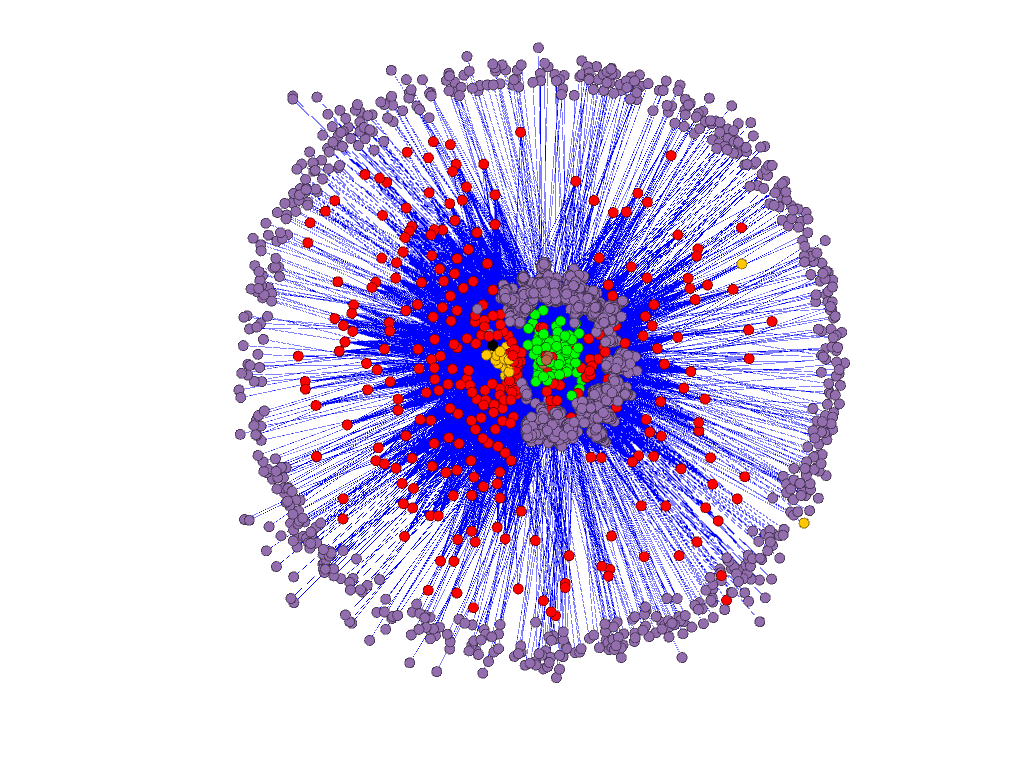
\includegraphics[scale=0.2, trim={0 0.5cm 0 6cm}]{Network_2011_forceAtlas.png}
	\caption{Visualization of the network for the year 2011. Nodes for this network are community(green), crime types(red), Schools(violet), Police stations(orange) and sanitations(brown).}
	\label{fig:fig1}
\end{figure}
Using results from similarity, we grouped communities in Chicago city. Below(Figures: \ref{fig:similarity_2011} - \ref{fig:similarity_2014}) are maps of Chicago with communities grouped according to the similarity measure for the years form 2011 to 2014.

\begin{figure}[!htb]
\minipage{0.5\textwidth}
  
\includegraphics[width=\linewidth]{my_similarity_2011.png}
  \caption{Clustering Community 2011}\label{fig:similarity_2011}
\endminipage\hfill
\minipage{0.5\textwidth}
  
\includegraphics[width=\linewidth]{my_similarity_2012.png}
  \caption{Clustering Community 2012}\label{fig:similarity_2012}
\endminipage\hfill
\minipage{0.5\textwidth}%
  
\includegraphics[width=\linewidth]{my_similarity_2013.png}
  \caption{Clustering Community 2013}\label{fig:similarity_2013}
\endminipage
\minipage{0.5\textwidth}%
  
\includegraphics[width=\linewidth]{my_similarity_2014.png}
  \caption{Clustering Community 2014}\label{fig:similarity_2014}
\endminipage
\caption{Similar communities over the years}
\end{figure}

\paragraph{Regression}
We used polynomial regression to predict the crime patterns for the year 2015. We had 4 years of complete dataset to use for our prediction. As explained above, each community will have its own feature vector. This vector comprises of weights of edges from the community to other nodes. This feature vector is concatenated with feature vector from the most similar community. This way we input the values for the regression model. We trained the regression model on just homicide and sexual assault crimes. The plot shows the predicted and actual output for the year 2015 [Figure \ref{output}]. This shows that our model successfully captures the crime pattern of Chicago city.

\begin{figure}[H]
	\centering
	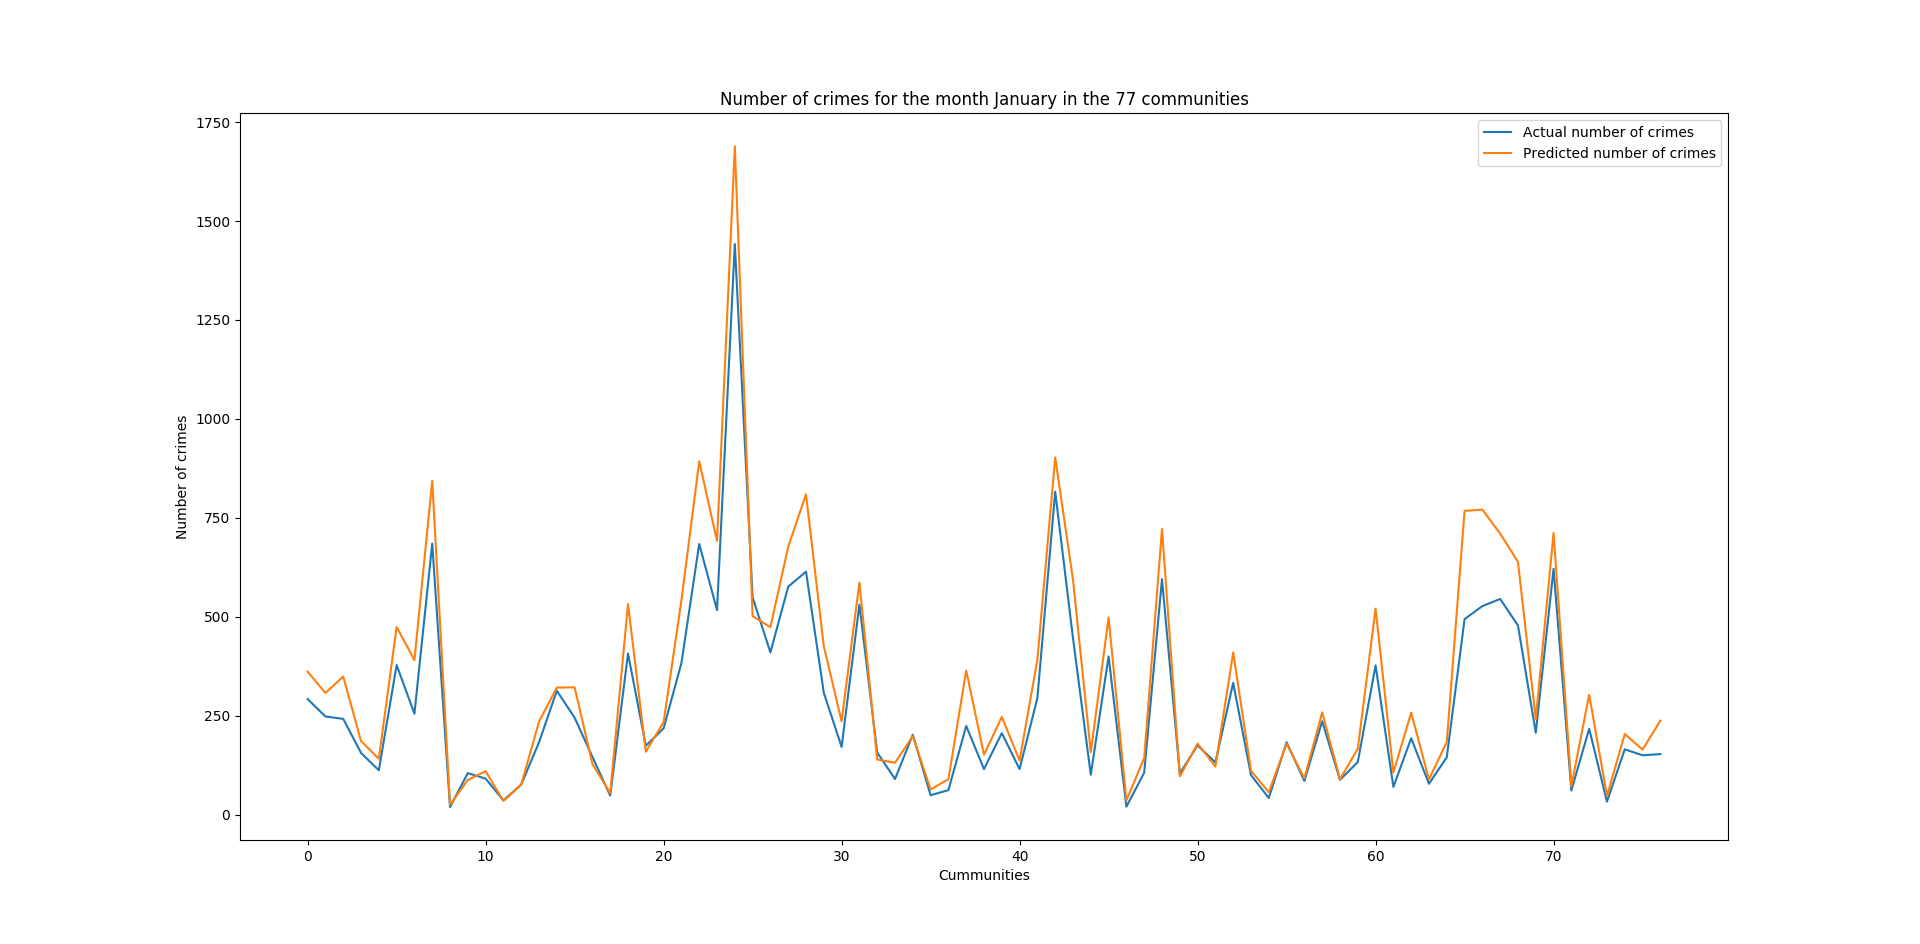
\includegraphics[trim={5cm, 1cm, 5cm, 1cm}, scale=0.3]{../Prediction/jan_predict.png}
	\caption{Actual and predicted number of crimes (homicide + sexual assault) for all 77 communities (for the month January)}
	\label{output}
\end{figure}

\section{Conclusion and Future Work}
We have done a comprehensive initial analysis of the dataset by analyzing it with the network analysis. We would still want to explore the data by using some new similarity technique. And we want to consider more than one similarity measure for preforming regression. We also want to try and connect different subnetworks in our network. We believe that by making the network more connected and by adding more sets of subsets to the network, we can predict the crime pattern better. To predict the crime patten for 2018, we need to regress for all input features such as number of visitors to the library, average ACT scores for 2018 etc. This needs more effort and we are hoping to continue this project next semester.

\begin{appendices}
 \chapter{Appendix A}
 \label{appendix:a}
 :Make network python code: 
 \lstinputlisting[language=Python]{"make_network.py"}
\end{appendices}
\newpage
\begin{thebibliography}{9}

\bibitem{role} Ahmed, N.~K., Rossi, R.~A., Willke, T.~L., \& Zhou, R.\ 2016, arXiv:1610.00844 
\bibitem{rwalk} F. Fouss, A. Pirotte, J. m. Renders and M. Saerens, "Random-Walk Computation of Similarities between Nodes of a Graph with Application to Collaborative Recommendation," in IEEE Transactions on Knowledge and Data Engineering, vol. 19, no. 3, pp. 355-369, March 2007.
\bibitem{data} \url{https://data.cityofchicago.org/Public-Safety/Crimes-2001-to-present/ijzp-q8t2}
\bibitem{police} \url{https://data.cityofchicago.org/Public-Safety/Chicago-Police-Department-Illinois-Uniform-Crime-R/c7ck-438e}
\bibitem{crime} \url{https://data.cityofchicago.org/Public-Safety/Crimes-2001-to-present/ijzp-q8t2}
\bibitem{library_loc}\url{https://data.cityofchicago.org/Education/Libraries-Locations-Hours-and-Contact-Information/x8fc-8rcq}
\bibitem{library_data} \url{https://data.cityofchicago.org/Education/Libraries-2011-Visitors-by-Location/xxwy-zyzu}
\bibitem{sanity} \url{https://data.cityofchicago.org/browse?q=311&sortBy=alpha&utf8=\%E2\%9C\%93}
\bibitem{police_stations} \url{https://data.cityofchicago.org/Public-Safety/Police-Stations/z8bn-74gv}
\bibitem{policeloc} \url{https://data.cityofchicago.org/Public-Safety/Boundaries-Police-Districts-current-/fthy-xz3r}
\bibitem{school} \url{https://data.cityofchicago.org/Education/Chicago-Public-Schools-Progress-Report-Cards-2011-/9xs2-f89t}
\end{thebibliography}
\end{document}